% Options for packages loaded elsewhere
\PassOptionsToPackage{unicode}{hyperref}
\PassOptionsToPackage{hyphens}{url}
%
\documentclass[
  ignorenonframetext,
]{beamer}
\usepackage{pgfpages}
\setbeamertemplate{caption}[numbered]
\setbeamertemplate{caption label separator}{: }
\setbeamercolor{caption name}{fg=normal text.fg}
\beamertemplatenavigationsymbolsempty
% Prevent slide breaks in the middle of a paragraph
\widowpenalties 1 10000
\raggedbottom
\setbeamertemplate{part page}{
  \centering
  \begin{beamercolorbox}[sep=16pt,center]{part title}
    \usebeamerfont{part title}\insertpart\par
  \end{beamercolorbox}
}
\setbeamertemplate{section page}{
  \centering
  \begin{beamercolorbox}[sep=12pt,center]{part title}
    \usebeamerfont{section title}\insertsection\par
  \end{beamercolorbox}
}
\setbeamertemplate{subsection page}{
  \centering
  \begin{beamercolorbox}[sep=8pt,center]{part title}
    \usebeamerfont{subsection title}\insertsubsection\par
  \end{beamercolorbox}
}
\AtBeginPart{
  \frame{\partpage}
}
\AtBeginSection{
  \ifbibliography
  \else
    \frame{\sectionpage}
  \fi
}
\AtBeginSubsection{
  \frame{\subsectionpage}
}

\usepackage{amsmath,amssymb}
\usepackage{iftex}
\ifPDFTeX
  \usepackage[T1]{fontenc}
  \usepackage[utf8]{inputenc}
  \usepackage{textcomp} % provide euro and other symbols
\else % if luatex or xetex
  \usepackage{unicode-math}
  \defaultfontfeatures{Scale=MatchLowercase}
  \defaultfontfeatures[\rmfamily]{Ligatures=TeX,Scale=1}
\fi
\usepackage{lmodern}
\usecolortheme{Flip}
\usefonttheme{serif} % use mainfont rather than sansfont for slide text
\useinnertheme{Flip}
\useoutertheme{Flip}
\ifPDFTeX\else  
    % xetex/luatex font selection
  \setmainfont[]{VisbyCF-Medium}
  \setsansfont[]{Latin Modern Sans}
  \setmathfont[]{Latin Modern Math}
\fi
% Use upquote if available, for straight quotes in verbatim environments
\IfFileExists{upquote.sty}{\usepackage{upquote}}{}
\IfFileExists{microtype.sty}{% use microtype if available
  \usepackage[]{microtype}
  \UseMicrotypeSet[protrusion]{basicmath} % disable protrusion for tt fonts
}{}
\makeatletter
\@ifundefined{KOMAClassName}{% if non-KOMA class
  \IfFileExists{parskip.sty}{%
    \usepackage{parskip}
  }{% else
    \setlength{\parindent}{0pt}
    \setlength{\parskip}{6pt plus 2pt minus 1pt}}
}{% if KOMA class
  \KOMAoptions{parskip=half}}
\makeatother
\usepackage{xcolor}
\newif\ifbibliography
\setlength{\emergencystretch}{3em} % prevent overfull lines
\setcounter{secnumdepth}{-\maxdimen} % remove section numbering

\usepackage{color}
\usepackage{fancyvrb}
\newcommand{\VerbBar}{|}
\newcommand{\VERB}{\Verb[commandchars=\\\{\}]}
\DefineVerbatimEnvironment{Highlighting}{Verbatim}{commandchars=\\\{\}}
% Add ',fontsize=\small' for more characters per line
\usepackage{framed}
\definecolor{shadecolor}{RGB}{241,243,245}
\newenvironment{Shaded}{\begin{snugshade}}{\end{snugshade}}
\newcommand{\AlertTok}[1]{\textcolor[rgb]{0.68,0.00,0.00}{#1}}
\newcommand{\AnnotationTok}[1]{\textcolor[rgb]{0.37,0.37,0.37}{#1}}
\newcommand{\AttributeTok}[1]{\textcolor[rgb]{0.40,0.45,0.13}{#1}}
\newcommand{\BaseNTok}[1]{\textcolor[rgb]{0.68,0.00,0.00}{#1}}
\newcommand{\BuiltInTok}[1]{\textcolor[rgb]{0.00,0.23,0.31}{#1}}
\newcommand{\CharTok}[1]{\textcolor[rgb]{0.13,0.47,0.30}{#1}}
\newcommand{\CommentTok}[1]{\textcolor[rgb]{0.37,0.37,0.37}{#1}}
\newcommand{\CommentVarTok}[1]{\textcolor[rgb]{0.37,0.37,0.37}{\textit{#1}}}
\newcommand{\ConstantTok}[1]{\textcolor[rgb]{0.56,0.35,0.01}{#1}}
\newcommand{\ControlFlowTok}[1]{\textcolor[rgb]{0.00,0.23,0.31}{#1}}
\newcommand{\DataTypeTok}[1]{\textcolor[rgb]{0.68,0.00,0.00}{#1}}
\newcommand{\DecValTok}[1]{\textcolor[rgb]{0.68,0.00,0.00}{#1}}
\newcommand{\DocumentationTok}[1]{\textcolor[rgb]{0.37,0.37,0.37}{\textit{#1}}}
\newcommand{\ErrorTok}[1]{\textcolor[rgb]{0.68,0.00,0.00}{#1}}
\newcommand{\ExtensionTok}[1]{\textcolor[rgb]{0.00,0.23,0.31}{#1}}
\newcommand{\FloatTok}[1]{\textcolor[rgb]{0.68,0.00,0.00}{#1}}
\newcommand{\FunctionTok}[1]{\textcolor[rgb]{0.28,0.35,0.67}{#1}}
\newcommand{\ImportTok}[1]{\textcolor[rgb]{0.00,0.46,0.62}{#1}}
\newcommand{\InformationTok}[1]{\textcolor[rgb]{0.37,0.37,0.37}{#1}}
\newcommand{\KeywordTok}[1]{\textcolor[rgb]{0.00,0.23,0.31}{#1}}
\newcommand{\NormalTok}[1]{\textcolor[rgb]{0.00,0.23,0.31}{#1}}
\newcommand{\OperatorTok}[1]{\textcolor[rgb]{0.37,0.37,0.37}{#1}}
\newcommand{\OtherTok}[1]{\textcolor[rgb]{0.00,0.23,0.31}{#1}}
\newcommand{\PreprocessorTok}[1]{\textcolor[rgb]{0.68,0.00,0.00}{#1}}
\newcommand{\RegionMarkerTok}[1]{\textcolor[rgb]{0.00,0.23,0.31}{#1}}
\newcommand{\SpecialCharTok}[1]{\textcolor[rgb]{0.37,0.37,0.37}{#1}}
\newcommand{\SpecialStringTok}[1]{\textcolor[rgb]{0.13,0.47,0.30}{#1}}
\newcommand{\StringTok}[1]{\textcolor[rgb]{0.13,0.47,0.30}{#1}}
\newcommand{\VariableTok}[1]{\textcolor[rgb]{0.07,0.07,0.07}{#1}}
\newcommand{\VerbatimStringTok}[1]{\textcolor[rgb]{0.13,0.47,0.30}{#1}}
\newcommand{\WarningTok}[1]{\textcolor[rgb]{0.37,0.37,0.37}{\textit{#1}}}

\providecommand{\tightlist}{%
  \setlength{\itemsep}{0pt}\setlength{\parskip}{0pt}}\usepackage{longtable,booktabs,array}
\usepackage{calc} % for calculating minipage widths
\usepackage{caption}
% Make caption package work with longtable
\makeatletter
\def\fnum@table{\tablename~\thetable}
\makeatother
\usepackage{graphicx}
\makeatletter
\def\maxwidth{\ifdim\Gin@nat@width>\linewidth\linewidth\else\Gin@nat@width\fi}
\def\maxheight{\ifdim\Gin@nat@height>\textheight\textheight\else\Gin@nat@height\fi}
\makeatother
% Scale images if necessary, so that they will not overflow the page
% margins by default, and it is still possible to overwrite the defaults
% using explicit options in \includegraphics[width, height, ...]{}
\setkeys{Gin}{width=\maxwidth,height=\maxheight,keepaspectratio}
% Set default figure placement to htbp
\makeatletter
\def\fps@figure{htbp}
\makeatother

\usepackage{tabu}
\usepackage{mathtools}
\usepackage{mathrsfs}
\makeatletter
\makeatother
\makeatletter
\makeatother
\makeatletter
\@ifpackageloaded{caption}{}{\usepackage{caption}}
\AtBeginDocument{%
\ifdefined\contentsname
  \renewcommand*\contentsname{Table of contents}
\else
  \newcommand\contentsname{Table of contents}
\fi
\ifdefined\listfigurename
  \renewcommand*\listfigurename{List of Figures}
\else
  \newcommand\listfigurename{List of Figures}
\fi
\ifdefined\listtablename
  \renewcommand*\listtablename{List of Tables}
\else
  \newcommand\listtablename{List of Tables}
\fi
\ifdefined\figurename
  \renewcommand*\figurename{Figure}
\else
  \newcommand\figurename{Figure}
\fi
\ifdefined\tablename
  \renewcommand*\tablename{Table}
\else
  \newcommand\tablename{Table}
\fi
}
\@ifpackageloaded{float}{}{\usepackage{float}}
\floatstyle{ruled}
\@ifundefined{c@chapter}{\newfloat{codelisting}{h}{lop}}{\newfloat{codelisting}{h}{lop}[chapter]}
\floatname{codelisting}{Listing}
\newcommand*\listoflistings{\listof{codelisting}{List of Listings}}
\makeatother
\makeatletter
\@ifpackageloaded{caption}{}{\usepackage{caption}}
\@ifpackageloaded{subcaption}{}{\usepackage{subcaption}}
\makeatother
\makeatletter
\@ifpackageloaded{tcolorbox}{}{\usepackage[skins,breakable]{tcolorbox}}
\makeatother
\makeatletter
\@ifundefined{shadecolor}{\definecolor{shadecolor}{rgb}{.97, .97, .97}}
\makeatother
\makeatletter
\makeatother
\makeatletter
\makeatother
\ifLuaTeX
  \usepackage{selnolig}  % disable illegal ligatures
\fi
\IfFileExists{bookmark.sty}{\usepackage{bookmark}}{\usepackage{hyperref}}
\IfFileExists{xurl.sty}{\usepackage{xurl}}{} % add URL line breaks if available
\urlstyle{same} % disable monospaced font for URLs
\hypersetup{
  pdftitle={Sélection de variables},
  pdfauthor={Léo Belzile},
  hidelinks,
  pdfcreator={LaTeX via pandoc}}

\title{Sélection de variables}
\subtitle{Analyse multidimensionnelle appliquée}
\author{Léo Belzile}
\date{}
\institute{HEC Montréal}

\begin{document}
\frame{\titlepage}
\ifdefined\Shaded\renewenvironment{Shaded}{\begin{tcolorbox}[sharp corners, interior hidden, breakable, borderline west={3pt}{0pt}{shadecolor}, boxrule=0pt, frame hidden, enhanced]}{\end{tcolorbox}}\fi

\begin{frame}{Modèles prédictifs}
\protect\hypertarget{moduxe8les-pruxe9dictifs}{}
\textbf{Objectif}: bâtir un modèle pour une variable réponse \(Y\) en
fonction de variables explicatives
\(\mathrm{X}_1, \ldots, \mathrm{X}_p\).

On s'intéresse à
\[\underset{\text{vraie moyenne inconnue}}{f(\mathrm{X}_1, \ldots, \mathrm{X}_p)}.\]

L'analyste détermine
\[\underset{\text{approximation}}{\widehat{f}(\mathrm{X}_1, \ldots, \mathrm{X}_p)},\]
une fonction des variables explicatives.
\end{frame}

\begin{frame}{Rappels sur la régression linéaire}
\protect\hypertarget{rappels-sur-la-ruxe9gression-linuxe9aire}{}
On spécifie que la \textbf{moyenne} de la variable réponse \(Y\) est une
fonction linéaire des variables explicatives
\(\mathrm{X}_1, \ldots, \mathrm{X}_p\), soit

\[\underset{\text{moyenne théorique}}{\mathsf{E}(Y \mid \mathbf{X})} = \underset{\text{
somme pondérée des variables explicatives}}{\beta_0 + \beta_1 \mathrm{X}_{i1} + \cdots + \beta_p \mathrm{X}_{ip}}.\]

en supposant que l'écart entre les observations et cette moyenne est
constant, \[\mathsf{Va}(Y \mid \mathbf{X}) = \sigma^2.\]
\end{frame}

\begin{frame}{Représentation alternative}
\protect\hypertarget{repruxe9sentation-alternative}{}
Pour la \(i\)e observation,

\[\underset{\text{réponse}}{Y_i} = \underset{\text{prédicteur linéaire}}{\beta_0 + \beta_1 \mathrm{X}_{i1} + \cdots + \beta_p \mathrm{X}_{ip}} + \underset{\text{aléa}}{\varepsilon_i}.\]

\begin{itemize}
\tightlist
\item
  L'aléa \(\varepsilon_i\) représente la distance \textbf{verticale}
  entre la vraie pente et l'observation
\item
  Autant d'aléas que d'observations (\(n\)), variable aléatoire
  inconnue\ldots{}
\end{itemize}
\end{frame}

\begin{frame}{Postulats}
\protect\hypertarget{postulats}{}
\begin{itemize}
\tightlist
\item
  L'aléa \(\varepsilon_i\) représente l'erreur, soit la différence entre
  la valeur observée et la moyenne de la population pour les même
  valeurs des variables explicatives.
\item
  On suppose que le modèle pour la moyenne est correctement spécifié:
  l'aléa a une moyenne théorique nulle, \(\mathsf{E}(\varepsilon_i)=0\).
\item
  On suppose que les observations sont indépendantes les unes des
  autres.
\end{itemize}
\end{frame}

\begin{frame}{Régression linéaire en deux dimensions}
\protect\hypertarget{ruxe9gression-linuxe9aire-en-deux-dimensions}{}
Si \(\mathsf{E}(Y)=\beta_0 + \beta_1 \mathrm{X}\), alors

\begin{itemize}
\tightlist
\item
  \(\beta_0\) représente l'ordonnée à l'origine (valeur quand
  \(\mathrm{X}=0\).)
\item
  \(\beta_1\) est la pente
\end{itemize}

\begin{figure}

{\centering \includegraphics[width=0.75\textwidth,height=\textheight]{MATH60602-diapos3_files/figure-beamer/unnamed-chunk-1-1.pdf}

}

\end{figure}
\end{frame}

\begin{frame}{Résidus ordinaires}
\protect\hypertarget{ruxe9sidus-ordinaires}{}
L'estimation des paramètres
\(\widehat{\beta}_0, \cdots, \widehat{\beta}_p\) nous donne
\[\underset{\text{prédiction}}{\widehat{Y}_i} = \widehat{\beta}_0 + \widehat{\beta}_1\mathrm{X}_{i1} \cdots + \widehat{\beta}_p\mathrm{X}_{ip}.\]

On peut approximer l'aléa à l'aide du \textbf{résidu ordinaire}, soit
\[\underset{\text{résidu ordinaire}}{e_i} = \underset{\text{observation}}{Y_i} - \underset{\text{prédiction}}{\widehat{Y}_i}.\]

\begin{itemize}
\tightlist
\item
  par construction, la moyenne des \(e_i\) est zéro.
\item
  le résidu ordinaire est la distance verticale entre l'observation et
  la ``droite'' \textbf{ajustée}
\end{itemize}
\end{frame}

\begin{frame}{Illustration des résidus ordinaires}
\protect\hypertarget{illustration-des-ruxe9sidus-ordinaires}{}
\begin{figure}

{\centering \includegraphics[width=0.8\textwidth,height=\textheight]{MATH60602-diapos3_files/figure-beamer/distancevert-1.pdf}

}

\end{figure}
\end{frame}

\begin{frame}{Erreur quadratique moyenne}
\protect\hypertarget{erreur-quadratique-moyenne}{}
L'erreur quadratique moyenne théorique est

\[\mathsf{E} \left[\left\{Y - \widehat{f}(\mathrm{X}_1, \ldots, \mathrm{X}_p)\right\}^2\right],\]
la moyenne de la différence au carré entre la vraie valeur de \(Y\) et
la valeur prédite par le modèle.

En pratique, on remplace la moyenne théorique par une moyenne empirique
obtenue à partir d'un échantillon aléatoire.
\end{frame}

\begin{frame}{Estimation des paramètres}
\protect\hypertarget{estimation-des-paramuxe8tres}{}
Comment estimer les paramètres \(\beta_0, \ldots, \beta_p\)?

\textbf{Optimisation}: trouver les valeurs qui minimisent l'erreur
quadratique moyenne \textbf{empirique} avec l'échantillon des \(n\)
observations, soit

\[\frac{e_1^2 + \cdots + e_n^2}{n}\]

Il existe une solution explicite au problème d'optimisation!
\end{frame}

\begin{frame}[fragile]{Estimation dans \textbf{R}}
\protect\hypertarget{estimation-dans-r}{}
La fonction \texttt{lm} calcule l'ajustement du modèle linéaire.

Arguments:

\begin{itemize}
\tightlist
\item
  \texttt{formula}: formule de type
  \texttt{reponse\ \textasciitilde{}\ \ variables\ explicatives}, où les
  variables explicatives sont séparées par un signe \texttt{+}
\item
  \texttt{data}: base de données
\end{itemize}

\begin{Shaded}
\begin{Highlighting}[numbers=left,,]
\NormalTok{modlin }\OtherTok{\textless{}{-}} \FunctionTok{lm}\NormalTok{(mpg }\SpecialCharTok{\textasciitilde{}}\NormalTok{ hp }\SpecialCharTok{+}\NormalTok{ wt, }
             \AttributeTok{data =}\NormalTok{ mtcars)}
\FunctionTok{summary}\NormalTok{(modlin)}
\end{Highlighting}
\end{Shaded}
\end{frame}

\begin{frame}[fragile]{Sortie de \texttt{summary}}
\protect\hypertarget{sortie-de-summary}{}
\footnotesize

\begin{verbatim}

Call:
lm(formula = mpg ~ hp + wt, data = mtcars)

Residuals:
   Min     1Q Median     3Q    Max 
-3.941 -1.600 -0.182  1.050  5.854 

Coefficients:
            Estimate Std. Error t value Pr(>|t|)    
(Intercept) 37.22727    1.59879  23.285  < 2e-16 ***
hp          -0.03177    0.00903  -3.519  0.00145 ** 
wt          -3.87783    0.63273  -6.129 1.12e-06 ***
---
Signif. codes:  0 '***' 0.001 '**' 0.01 '*' 0.05 '.' 0.1 ' ' 1

Residual standard error: 2.593 on 29 degrees of freedom
Multiple R-squared:  0.8268,    Adjusted R-squared:  0.8148 
F-statistic: 69.21 on 2 and 29 DF,  p-value: 9.109e-12
\end{verbatim}

\normalsize
\end{frame}

\begin{frame}{Tableau de sortie}
\protect\hypertarget{tableau-de-sortie}{}
\begin{itemize}
\tightlist
\item
  Formule de l'appel
\item
  Statistiques descriptives des résidus ordinaires \(e_1, \ldots, e_n\).
\item
  Tableau des estimations

  \begin{itemize}
  \tightlist
  \item
    Coefficients \(\widehat{\beta}_j\)
  \item
    Erreurs-types, \(\mathsf{se}(\widehat{\beta}_j)\)
  \item
    Statistique du test-\emph{t} pour \(\mathscr{H}_0: \beta_j=0\), soit
    \(t=\widehat{\beta}_j/\mathsf{se}(\widehat{\beta}_j)\)
  \item
    Valeur-\emph{p} selon loi nulle \(\mathsf{St}(n-p-1)\)
  \end{itemize}
\item
  Estimation de l'écart-type \(\widehat{\sigma}\) et degrés de liberté
  \(n-p-1\)
\item
  Estimations du coefficient de détermination, \(R^2\) et \(R^2\) ajusté
\item
  Statistique \(F\) d'ajustement global et valeur-\(p\) de
  \(\mathsf{F}(p, n - p - 1)\)

  \begin{itemize}
  \tightlist
  \item
    \(\mathscr{H}_a\): modèle linéaire
  \item
    \(\mathscr{H}_0\): modèle avec uniquement ordonnée à l'origine
    (chaque observation prédite par la moyenne des réponses,
    \(\overline{Y}\))
  \end{itemize}
\end{itemize}

\normalsize
\end{frame}

\begin{frame}[fragile]{Quelques méthodes pour \texttt{lm}}
\protect\hypertarget{quelques-muxe9thodes-pour-lm}{}
\begin{itemize}
\tightlist
\item
  \texttt{resid} pour les résidus ordinaires \(e_i\)
\item
  \texttt{fitted} pour les valeurs ajustées \(\widehat{Y}_i\)
\item
  \texttt{coef} pour les estimations des paramètres
  \(\widehat{\beta}_0, \ldots, \widehat{\beta}_p\)
\item
  \texttt{plot} pour des diagnostics graphiques d'ajustement
\item
  \texttt{anova} pour la comparaison de modèles emboîtés
\item
  \texttt{predict} pour les prédictions (avec nouvelles données)
\item
  \texttt{confint} pour intervalles de confiance pour les paramètres.
\end{itemize}
\end{frame}

\begin{frame}[fragile]{Variables catégorielles}
\protect\hypertarget{variables-catuxe9gorielles}{}
\begin{itemize}
\tightlist
\item
  Les facteurs (\texttt{\textless{}factor\textgreater{}}) sont traités
  adéquatement par \textbf{R}.
\item
  Si la variable a \(K\) valeurs possibles (niveaux), le modèle inclut
  \(K-1\) indicatrices 0/1.
\item
  Par défaut dans \textbf{R}, la catégorie de référence est la plus
  petite en ordre alphanumérique.
\end{itemize}
\end{frame}

\begin{frame}[fragile]{Encodage des variables catégorielles}
\protect\hypertarget{encodage-des-variables-catuxe9gorielles}{}
Considérons une variable catégorielle \texttt{cat} avec niveaux
\texttt{1}, \texttt{2}, et \texttt{3}.

\begin{longtable}[]{@{}ccc@{}}
\toprule\noalign{}
\texttt{cat} & \texttt{cat2} & \texttt{cat3} \\
\midrule\noalign{}
\endhead
1 & 0 & 0 \\
2 & 1 & 0 \\
3 & 0 & 1 \\
\bottomrule\noalign{}
\end{longtable}

La catégorie de référence est associée à l'ordonnée à l'origine (quand
\texttt{cat2=0} et \texttt{cat3=0}).
\end{frame}

\begin{frame}[fragile]{Sélection de variables et de modèles}
\protect\hypertarget{suxe9lection-de-variables-et-de-moduxe8les}{}
\begin{itemize}
\tightlist
\item
  Comment choisir quelles variables inclure?
\item
  Quel est la spécification adéquate pour
  \(f(\mathrm{X}_1, \ldots, \mathrm{X}_p)\)?

  \begin{itemize}
  \tightlist
  \item
    régression, réseaux de neurone, forêts aléatoires, etc.
  \item
    transformations de variables, \texttt{age}\({}^2\),
    \(\ln(\)\texttt{age}\()\), etc.
  \end{itemize}
\end{itemize}

Notre but sera de sélectionner un \textbf{bon} modèle, selon les
objectifs de l'étude
\end{frame}

\begin{frame}{Prédiction vs inférence}
\protect\hypertarget{pruxe9diction-vs-infuxe9rence}{}
\textbf{Prédiction}: obtenir une estimation de \(\widehat{Y}\): on veut
un modèle performant

\textbf{Inférence}: estimer l'effet de variables explicatives, effectuer
des tests d'hypothèses

Pour l'inférence, il est préférable de spécifier le modèle dès le départ
(devis expérimental) selon des considérations scientifiques et de s'y
tenir.
\end{frame}

\begin{frame}{Spécification adéquate d'un modèle}
\protect\hypertarget{spuxe9cification-aduxe9quate-dun-moduxe8le}{}
\begin{block}{Démonstration \textbf{R}}
\protect\hypertarget{duxe9monstration-r}{}
\begin{itemize}
\tightlist
\item
  Omettre des termes importants mène à un \textbf{modèle biaisé}.
\item
  Ajouter des termes superflus augmente la \textbf{variabilité} (on
  estime des zéros).
\end{itemize}
\end{block}
\end{frame}

\begin{frame}{Évaluer la performance d'un modèle}
\protect\hypertarget{uxe9valuer-la-performance-dun-moduxe8le}{}
On peut calculer l'erreur quadratique moyenne (EQM) sur l'ensemble des
données qui servent à ajuster le modèle.

Q: Est-ce que c'est un marqueur fiable de la performance du modèle?
\end{frame}

\begin{frame}[fragile]{Exemple avec la régression polynomiale}
\protect\hypertarget{exemple-avec-la-ruxe9gression-polynomiale}{}
On a simulé des observations d'un modèle polynomiale d'ordre \(K\), de
la forme
\[\mathsf{E}(Y \mid \mathbf{X}) = \beta_0 + \beta_1 \mathrm{X} + \cdots + \beta_K \mathrm{X}^K.\]

On vise à estimer l'ordre du polynôme en effectuant des régressions
linéaires.

\begin{Shaded}
\begin{Highlighting}[numbers=left,,]
\FunctionTok{data}\NormalTok{(polynome, }\AttributeTok{package =} \StringTok{"hecmulti"}\NormalTok{)}
\NormalTok{k }\OtherTok{\textless{}{-}}\NormalTok{ 4L }\CommentTok{\# degré du polynôme}
\FunctionTok{lm}\NormalTok{(y }\SpecialCharTok{\textasciitilde{}} \FunctionTok{poly}\NormalTok{(x, }\AttributeTok{degree =}\NormalTok{ k), }
   \AttributeTok{data =}\NormalTok{ polynome)}
\end{Highlighting}
\end{Shaded}
\end{frame}

\begin{frame}{Aperçu des données}
\protect\hypertarget{aperuxe7u-des-donnuxe9es}{}
\begin{figure}

{\centering \includegraphics[width=0.7\textwidth,height=\textheight]{MATH60602-diapos3_files/figure-beamer/unnamed-chunk-5-1.pdf}

}

\end{figure}

D'après vous, quelle est la vraie valeur de \(K\)?
\end{frame}

\begin{frame}{Ajustement de polynômes}
\protect\hypertarget{ajustement-de-polynuxf4mes}{}
\begin{figure}

{\centering \includegraphics[width=0.8\textwidth,height=\textheight]{MATH60602-diapos3_files/figure-beamer/unnamed-chunk-6-1.pdf}

}

\end{figure}

Ajustement pour des polynômes de degré \(K=1, 4, 10\).
\end{frame}

\begin{frame}[fragile]{Évaluation de la performance}
\protect\hypertarget{uxe9valuation-de-la-performance}{}
Pour \(K=1, \ldots, 10\):

\begin{itemize}
\tightlist
\item
  Ajuster le modèle linéaire
\item
  Obtenir les résidus ordinaires
\item
  Calculer l'erreur quadratique moyenne
\end{itemize}

\begin{Shaded}
\begin{Highlighting}[numbers=left,,]
\FunctionTok{data}\NormalTok{(polynome, }\AttributeTok{package =} \StringTok{"hecmulti"}\NormalTok{)}
\NormalTok{eqm }\OtherTok{\textless{}{-}} \FunctionTok{vector}\NormalTok{(}\AttributeTok{length =}\NormalTok{ 10L, }\AttributeTok{mode =} \StringTok{"numeric"}\NormalTok{)}
\ControlFlowTok{for}\NormalTok{(K }\ControlFlowTok{in} \FunctionTok{seq\_len}\NormalTok{(}\DecValTok{10}\NormalTok{))\{}
\NormalTok{ mod }\OtherTok{\textless{}{-}} \FunctionTok{lm}\NormalTok{(y }\SpecialCharTok{\textasciitilde{}} \FunctionTok{poly}\NormalTok{(x, }\AttributeTok{degree =}\NormalTok{ K), }\AttributeTok{data =}\NormalTok{ polynome)}
\NormalTok{ eqm[K] }\OtherTok{\textless{}{-}} \FunctionTok{mean}\NormalTok{(}\FunctionTok{resid}\NormalTok{(mod)}\SpecialCharTok{\^{}}\DecValTok{2}\NormalTok{)}
\NormalTok{\}}
\end{Highlighting}
\end{Shaded}
\end{frame}

\begin{frame}{Estimation de l'erreur quadratique moyenne}
\protect\hypertarget{estimation-de-lerreur-quadratique-moyenne}{}
\begin{figure}

{\centering \includegraphics[width=0.7\textwidth,height=\textheight]{MATH60602-diapos3_files/figure-beamer/unnamed-chunk-8-1.pdf}

}

\end{figure}

Plus le modèle est complexe, plus l'erreur quadratique moyenne de
l'échantillon d'apprentissage est petite!
\end{frame}

\begin{frame}{Suroptimisme}
\protect\hypertarget{suroptimisme}{}
L'erreur quadratique moyenne décroît mécaniquement à chaque fois qu'on
ajoute une variable au modèle de régression.

C'est pourquoi on ne peut pas l'utiliser comme outil de sélection de
variables, autrement on va surestimer la performance
(\textbf{suroptimisme}).
\end{frame}

\begin{frame}{Surajustement}
\protect\hypertarget{surajustement}{}
Un modèle plus complexe va toujours mieux s'ajuster aux données de
l'échantillon.

En revanche, il se \textbf{généralise} moins bien (notre objectif en
prédiction).

\begin{figure}

{\centering \includegraphics[width=0.7\textwidth,height=\textheight]{MATH60602-diapos3_files/figure-beamer/overfitting-1.pdf}

}

\end{figure}
\end{frame}

\begin{frame}{Morale de l'histoire}
\protect\hypertarget{morale-de-lhistoire}{}
Nous nous sommes rendus coupables d'un péché capital en utilisant deux
fois les données

\begin{itemize}
\tightlist
\item
  une fois pour l'ajustement,
\item
  une fois pour la validation.
\end{itemize}

C'est comme tremper deux fois un biscuit dans le verre de lait\ldots{}
\end{frame}

\begin{frame}{Estimation fiable de la performance}
\protect\hypertarget{estimation-fiable-de-la-performance}{}
\begin{itemize}
\tightlist
\item
  Pénalisation de la complexité du modèle

  \begin{itemize}
  \tightlist
  \item
    critères d'information
  \item
    pénalité sur les coefficients (\emph{ridge}, LASSO)
  \end{itemize}
\item
  Validation et entraînement avec des données différentes

  \begin{itemize}
  \tightlist
  \item
    validation externe
  \item
    validation croisée
  \end{itemize}
\end{itemize}
\end{frame}

\begin{frame}{Pénalisation}
\protect\hypertarget{puxe9nalisation}{}
Utiliser toutes les données (échantillon de validation), mais ajouter
une pénalité.

Si le modèle est ajusté avec la méthode du maximum de vraisemblance,
alors on a accès aux critères d'information.
\end{frame}

\begin{frame}{Lien entre régression linéaire et vraisemblance}
\protect\hypertarget{lien-entre-ruxe9gression-linuxe9aire-et-vraisemblance}{}
Si on suppose que les aléas sont indépendants et suivent une loi normale
de variance \(\sigma^2\) constante, alors la log-vraisemblance s'écrit

\begin{align*}
\ell(\boldsymbol{Y}; \mathbf{X}, \boldsymbol{\beta}, \sigma) & = -\frac{n}{2}\ln(2\pi) -n\ln(\sigma) \\&\quad - \frac{1}{2\sigma^2}\sum_{i=1}^n (Y_i - \beta_0 - \cdots - \mathrm{X}_{ip}\beta_p)^2.
\end{align*}

Ainsi, l'estimateur des moindres carrés,
\(\widehat{\boldsymbol{\beta}}\), correspond au maximum de vraisemblance
des coefficients.
\end{frame}

\begin{frame}{Critères d'information}
\protect\hypertarget{crituxe8res-dinformation}{}
Valables uniquement pour les modèles ajustés par \textbf{maximum de
vraisemblance}, ils sont de la forme

\begin{align*}
\mathsf{IC} &= -\text{ajustement} + \text{pénalité} \times\text{nb param} \\
\end{align*}

\begin{itemize}
\tightlist
\item
  On veut maximiser l'ajustement, donc minimiser le premier terme.
\item
  La pénalité vient contrebalancer l'amélioration mécanique de
  l'ajustement quand le modèle a plus de flexibilité.
\item
  Plus le critère d'information est petit, meilleur c'est.
\end{itemize}
\end{frame}

\begin{frame}{Critères d'information}
\protect\hypertarget{crituxe8res-dinformation-1}{}
Pour la régression linéaire, on peut réécrire les critères d'information
sous la forme \begin{align*}
\mathsf{AIC} &=n \ln (\widehat{\mathsf{EQM}}) +2\times \text{nb param}+ \text{constante},\\
\mathsf{AIC} &=n \ln (\widehat{\mathsf{EQM}}) +\ln(n)\times \text{nb param}+ \text{constante},
\end{align*}

\begin{itemize}
\item
  Le critère d'Akaike (\(\text{AIC}\)) utilise une pénalité de 2, le
  critère bayésien (\(\text{BIC}\)) de \(\ln(n)\).
\item
  Le \(\mathsf{BIC}\) (critère Bayésien de Schwarz) pénalise donc
  davantage que le \(\mathsf{AIC}\) (critère d'Akaike).
\end{itemize}
\end{frame}

\begin{frame}[fragile]{Utiliser les critères d'information}
\protect\hypertarget{utiliser-les-crituxe8res-dinformation}{}
\begin{itemize}
\tightlist
\item
  Plus la valeur du critère d'information est petite, meilleure est
  l'adéquation (et donc la performance).
\item
  La pénalité assure que les modèles plus complexes ne sont pas
  systématiquement retournés.
\item
  Le \(\textsf{BIC}\) retourne toujours des modèles plus parcimonieux
  (c'est-à-dire avec moins de paramètres) que le \(\textsf{AIC}\).
\item
  Génériques \texttt{AIC} et \texttt{BIC} en \textbf{R}
\end{itemize}
\end{frame}

\begin{frame}{Illustration}
\protect\hypertarget{illustration}{}
\begin{figure}

{\centering \includegraphics[width=0.8\textwidth,height=\textheight]{MATH60602-diapos3_files/figure-beamer/fig-polynome-ajustement-1.pdf}

}

\caption{\label{fig-polynome-ajustement}Critères d'information en
fonction de l'ordre du polynôme.}

\end{figure}

Les deux critères d'information retournent \(K=3\) comme choix optimal.
\end{frame}

\begin{frame}{Séparation des données}
\protect\hypertarget{suxe9paration-des-donnuxe9es}{}
Ne pas utiliser les données employés pour ajuster un modèle pour
\textbf{prédire la performance}.

\begin{itemize}
\tightlist
\item
  échantillons d'apprentissage/validation/test (fixes)
\item
  validation croisée
\end{itemize}
\end{frame}

\begin{frame}{Validation externe}
\protect\hypertarget{validation-externe}{}
Séparer l'ensemble d'observations en plusieurs groupes

\begin{itemize}
\tightlist
\item
  l'échantillon d'apprentissage pour l'ajustement du modèle
\item
  l'échantillon de validation pour l'estimation de la performance
\item
  l'échantillon test pour l'inférence (optionnel)
\end{itemize}

En pratique, il faut beaucoup d'observations!
\end{frame}

\begin{frame}{Avantages et inconvénients de la validation externe}
\protect\hypertarget{avantages-et-inconvuxe9nients-de-la-validation-externe}{}
Applicable en toute généralité peu importe le type de modèle.

Cette approche, qui compartimente les échantillons, n'est pas sans
faille.

\begin{itemize}
\tightlist
\item
  On obtient un résultat différent selon la division
\item
  Gaspillage potentiel
\item
  Choix d'ordinaire aléatoire, mais choix particuliers de fenêtre selon
  données (par ex., séries chronologiques)
\end{itemize}
\end{frame}

\begin{frame}{Validation croisée}
\protect\hypertarget{validation-croisuxe9e}{}
Une autre méthode de rééchantillonage

Diviser l'échantillon en \(M\) groupes d'observations de taille moyenne
égale

\begin{itemize}
\tightlist
\item
  utiliser \(M-1\) groupes pour l'ajustement
\item
  estimer la performance avec les données du dernier groupe
\end{itemize}

Les regroupements sont aléatoires, tout comme la mesure finale de
performance!
\end{frame}

\begin{frame}{Étapes de la validation croisée à \(M\) groupes}
\protect\hypertarget{uxe9tapes-de-la-validation-croisuxe9e-uxe0-m-groupes}{}
\begin{enumerate}
\tightlist
\item
  Diviser l'échantillon au hasard en \(M\) parties
  \(P_1, P_2, \ldots, P_M\) contenant toutes à peu près le même nombre
  d'observations.
\item
  Pour \(j = 1\) à \(M\),

  \begin{enumerate}
  [i.]
  \tightlist
  \item
    Enlever la partie \(j\).
  \item
    Estimer les paramètres du modèle en utilisant les observations des
    \(M-1\) autres parties combinées.
  \item
    Calculer la mesure de performance (par exemple la somme du carré des
    erreurs \(\{Y_i - \widehat{Y}_i\}^2\)) de ce modèle pour le groupe
    \(P_j\).
  \end{enumerate}
\item
  Combiner les \(M\) estimations de performance pour obtenir une mesure
  de performance finale.
\end{enumerate}
\end{frame}

\begin{frame}{Illustration de la validation croisée}
\protect\hypertarget{illustration-de-la-validation-croisuxe9e}{}
\includegraphics[width=0.8\textwidth,height=\textheight]{MATH60602-diapos3_files/figure-beamer/validationcroiseeillust-1.pdf}
\end{frame}

\begin{frame}{Combien de groupes \(M\) pour la validation croisée?}
\protect\hypertarget{combien-de-groupes-m-pour-la-validation-croisuxe9e}{}
La validation croisée est plus coûteuse parce qu'on doit ajuster \(M\)
fois le modèles

\begin{itemize}
\tightlist
\item
  Pour la régression linéaire, choisir \(M=n\) (\emph{leave-one-out
  cross-validation}) permet d'éviter de réajuster le modèle grâce à un
  artifice de calcul.
\item
  On recommande habituellement de prendre \(\min\{n^{1/2}, 10\}\)
  groupes,
\item
  mais les choix \(M=5\) ou \(M=10\) sont ceux qui revient le plus
  souvent en pratique.
\end{itemize}

\footnotesize

Voir Davison \& Hinkley (1997), \emph{Bootstrap methods and their
applications}, Section 6.4 pour une discussion plus étoffée et
l'algorithme 6.5 pour une meilleure implémentation.

\normalsize
\end{frame}

\begin{frame}{Validation croisée = résultat aléatoire!}
\protect\hypertarget{validation-croisuxe9e-ruxe9sultat-aluxe9atoire}{}
Soit \(\widehat{\mathsf{EQM}}_{\text{VC}}\) l'estimation de l'erreur
quadratique moyenne obtenue par validation croisée à \(M\) plis pour un
modèle \(\mathcal{M}\) donné.

Si on a un nombre similaire d'observations dans chaque groupe:

\begin{itemize}
\tightlist
\item
  calculer l'erreur quadratique moyenne de chaque pli,
  \(\widehat{\mathsf{EQM}}_{\text{VC}, m}\)
\item
  si \(M\) est suffisamment grand (disons \(M \geq 10\)), on peut
  estimer l'écart-type empirique de ces moyennes
  \[ \mathsf{sd} = \frac{1}{M-1} \sum_{m=1}^{M} (\widehat{\mathsf{EQM}}_{\text{VC}, m}-\widehat{\mathsf{EQM}}_{\text{VC}})^2\]
\item
  Pour obtenir l'\textbf{erreur-type de la moyenne globale}, diviser par
  la racine de la taille du nombre de groupes, d'où
  \[\mathsf{se}(\widehat{\mathsf{EQM}}_{\text{VC}}) = \mathsf{sd}/\sqrt{M}\]
\end{itemize}
\end{frame}

\begin{frame}{Règle d'une erreur-type}
\protect\hypertarget{ruxe8gle-dune-erreur-type}{}
Soit \(\mathcal{M}_{\text{opt}}\) le modèle avec la plus petite erreur
quadratique moyenne de validation croisée.

Suivant Breiman, on choisit le modèle le plus simple qui soit à au plus
une erreur-type de la performance du modèle
\(\mathcal{M}_{\text{opt}}\), en prenant prend
\(\mathsf{se}\{\widehat{\mathsf{EQM}}_{\text{VC}}(\mathcal{M}_{\text{opt}})\}\).
\end{frame}

\begin{frame}{Illustration de la règle de une erreur-type}
\protect\hypertarget{illustration-de-la-ruxe8gle-de-une-erreur-type}{}
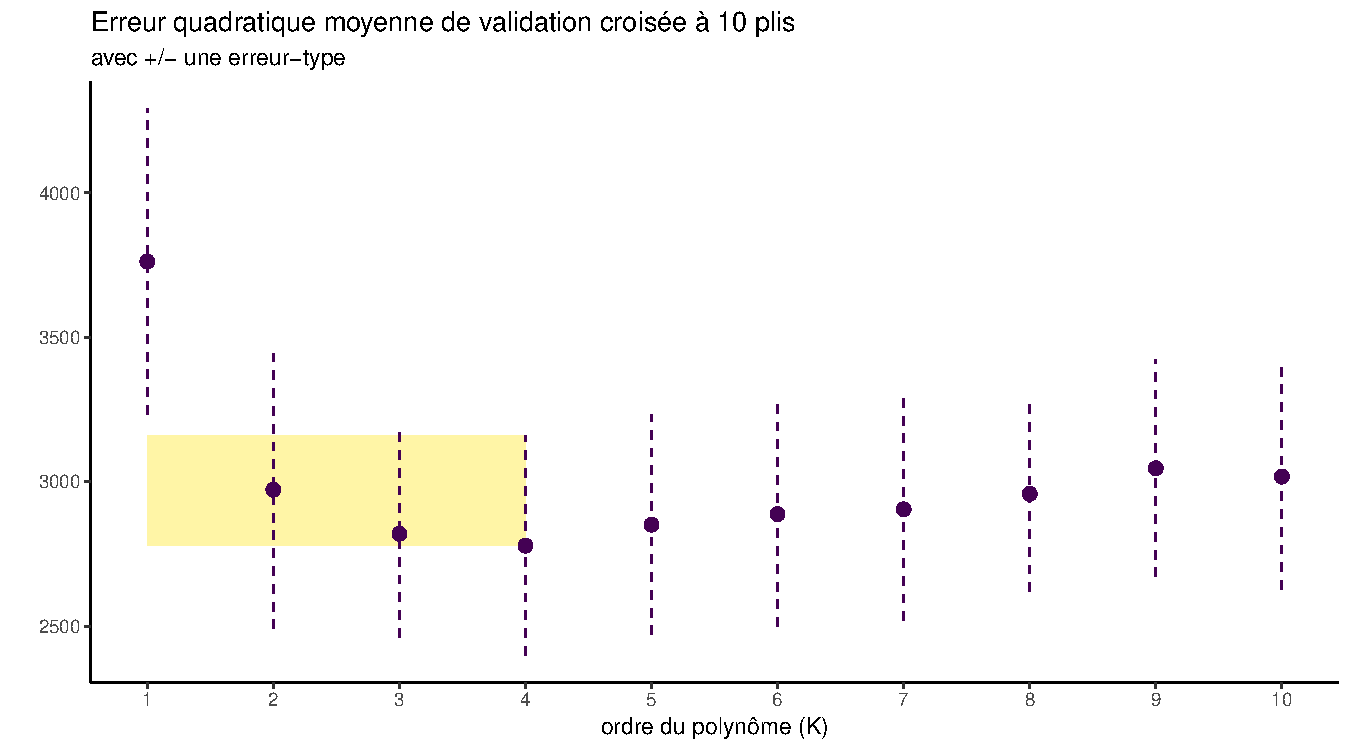
\includegraphics{figures/fig-validationcroisee-une-erreur-type.pdf}

La bande jaune donne une erreur-type du meilleur modèle. On choisirait
le modèle avec \(M=2\), plutôt que \(M=4\)
\end{frame}

\begin{frame}[fragile]{Validation croisée en \textbf{R}}
\protect\hypertarget{validation-croisuxe9e-en-r}{}
Le paquet \texttt{caret} a une fonction pour faire la validation
croisée.

\begin{Shaded}
\begin{Highlighting}[numbers=left,,]
\NormalTok{cv\_caret }\OtherTok{\textless{}{-}} 
\NormalTok{  caret}\SpecialCharTok{::}\FunctionTok{train}\NormalTok{(}\AttributeTok{form =} \FunctionTok{formula}\NormalTok{(y }\SpecialCharTok{\textasciitilde{}} \FunctionTok{poly}\NormalTok{(x, }\AttributeTok{degree =} \DecValTok{3}\NormalTok{)), }
             \AttributeTok{data =}\NormalTok{ polynome, }
             \AttributeTok{method =} \StringTok{"lm"}\NormalTok{,}
             \AttributeTok{trControl =}\NormalTok{ caret}\SpecialCharTok{::}\FunctionTok{trainControl}\NormalTok{(}
               \AttributeTok{method =} \StringTok{"cv"}\NormalTok{,}
               \AttributeTok{number =} \DecValTok{10}\NormalTok{)) }\CommentTok{\#nb plis}
\NormalTok{reqm\_cv }\OtherTok{\textless{}{-}}\NormalTok{ cv\_caret}\SpecialCharTok{$}\NormalTok{results}\SpecialCharTok{$}\NormalTok{RMSE }\CommentTok{\# racine EQM}
\NormalTok{reqm\_se\_cv }\OtherTok{\textless{}{-}}\NormalTok{ cv\_caret}\SpecialCharTok{$}\NormalTok{results}\SpecialCharTok{$}\NormalTok{RMSESD }\SpecialCharTok{/} \FunctionTok{sqrt}\NormalTok{(}\DecValTok{10}\NormalTok{) }
\CommentTok{\# calcul de l\textquotesingle{}erreur{-}type de la racine EMQ pour ce modèle}
\end{Highlighting}
\end{Shaded}

Aussi \texttt{boot::cv.glm()} qui inclut une correction de biais pour
les modèles linéaires généralisé.
\end{frame}

\begin{frame}{Résultats de la validation croisée}
\protect\hypertarget{ruxe9sultats-de-la-validation-croisuxe9e}{}
\begin{figure}

{\centering \includegraphics[width=1\textwidth,height=\textheight]{MATH60602-diapos3_files/figure-beamer/fig-plotcv-1.pdf}

}

\caption{\label{fig-plotcv}Boîtes à moustaches des 100 estimations de
l'erreur quadratique moyenne obtenues par validation croisée à 10 plis.}

\end{figure}
\end{frame}

\begin{frame}{Récapitulatif}
\protect\hypertarget{ruxe9capitulatif}{}
\begin{itemize}
\tightlist
\item
  Le choix de la complexité d'un modèle est un compromis entre

  \begin{itemize}
  \tightlist
  \item
    le biais (modèle trop simple, mal spécifié) et
  \item
    la variance (même nombre d'observations/budget, plus de paramètres à
    estimer, estimations moins fiables)
  \end{itemize}
\item
  L'erreur quadratique moyenne est la mesure usuelle de la performance
  d'un modèle linéaire
\end{itemize}
\end{frame}

\begin{frame}{Récapitulatif}
\protect\hypertarget{ruxe9capitulatif-1}{}
Si on estime la performance avec les mêmes données qui ont servi à
l'ajustement, on surestime la performance

\begin{itemize}
\tightlist
\item
  l'erreur quadratique moyenne calculée sur les mêmes données qui ont
  servi à l'entraînement est biaisée
\item
  cela mène à du \textbf{surajustement}
\end{itemize}
\end{frame}

\begin{frame}{Récapitulatif}
\protect\hypertarget{ruxe9capitulatif-2}{}
Trois méthodes pour estimer de manière plus objective la performance
d'un modèle

\begin{itemize}
\tightlist
\item
  Critères d'information (pénalisation)
\item
  Validation externe
\item
  Validation croisée
\end{itemize}

\footnotesize

Vous devez être en mesure de nommer les forces et faiblesses et
d'expliquer le fonctionnement (avec du pseudocode).
\end{frame}



\end{document}
